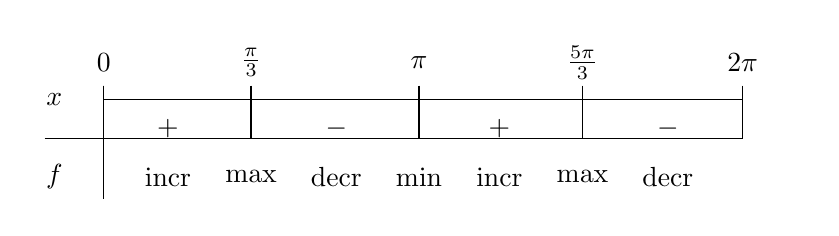
\begin{tikzpicture}
  \matrix[row sep=1mm,column sep=2mm,ampersand replacement=\&] {
    \& \node(tp1){$0$}; \&\& \node(tp2){$\frac\pi3$}; \&\& \node(tp3){$\pi$}; \&\& \node(tp4){$\frac{5\pi}3$}; \&\& \node(tp5){$2\pi$}; \\[-1ex]
    \node {$x$}; \& \node(linestart){}; \&\&\&\&\&\&\&\&\& \node(lineend) {}; \\[-1ex]
    \node(fpstart){$\fp$}; \&\& \node{$+$}; \&\& \node{$-$}; \&\& \node{$+$}; \&\& \node{$-$}; \\
    \node(fstart){$f$}; \&\& \node{incr}; \& \node{max}; \& \node{decr}; \& \node{min}; \& \node{incr}; \& \node{max}; \& \node{decr};\\
  };
  \draw (tp1 |- linestart) -- (tp5 |- lineend);
  \draw (fpstart.south west) -- (tp5 |- fpstart.south);
  \draw (tp1|-linestart)+(0,5pt) -- (tp1 |- fstart.south);
  \foreach \x in {1,2,3,4,5} {
    \draw (tp\x|-linestart)+(0,5pt) -- (tp\x |- fpstart.south);
  }
\end{tikzpicture}